%!TEX root = ../toolhinweise.tex

\section{YAKINDU Statechart Syntax}
\label{sec:syntax}

Statecharts können die gleichen Konstrukte abbilden wie UML Zustandsdiagramme.
YAKINDU SCT zielt auf die Ausführung von Statecharts ab und erzwingt deswegen eine präzisere und striktere Syntax, damit die Ausführung in jedem Fall eindeutig ist. 

Hier werden die wichtigsten Besonderheiten vorgestellt. Eine vollständige Spachreferenz befindet sich auf \url{https://www.itemis.com/en/yakindu/state-machine/documentation/user-guide/sclang_statechart_language_reference}.

\subsection{Zustände und Regionen}

Statecharts bestehen aus Regionen, die Zustände beinhalten können, die wiederum Regionen beinhalten können, die neue Zustände beinhalten können, und so weiter. Regionen werden dargestellt als hellgraue Rechtecke, Zustände als hellblaue abgerundete Rechtecke. 
Regionen können wie Zustände Namen haben, die Benennung ist aber optional. 
Ein Zustand, der Regionen beinhaltet, kann dennoch lokale Reaktionen haben. 
Wenn innerhalb eines Zustandes mehrere (orthogonale) Regionen sind müssen Sie eine explizite (Ausführungs-)Reihenfolge haben.

\begin{center}
	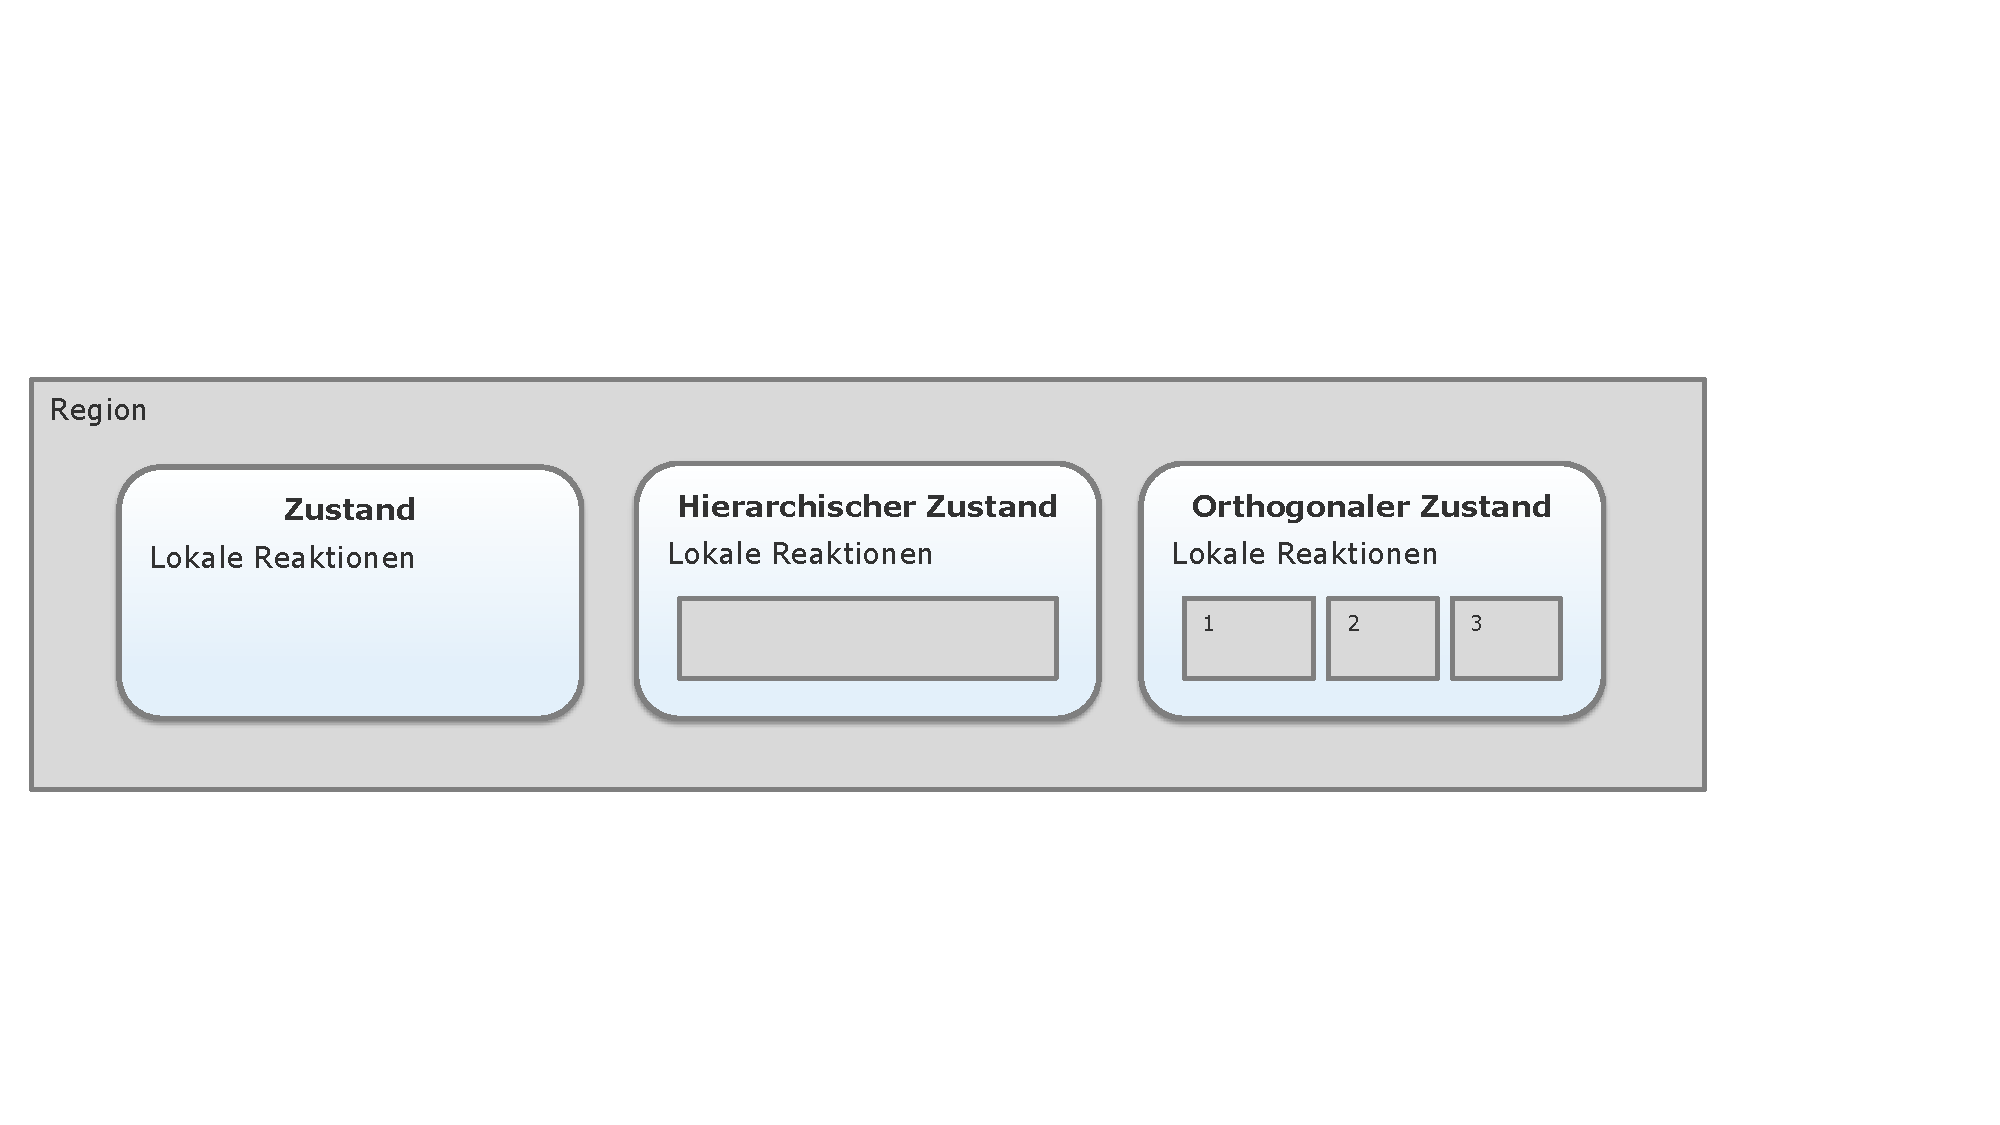
\includegraphics[width=0.8\textwidth]{syntax_regionen}
\end{center}

Bei UML-Zustandsdiagrammen sind Regionen ebenfalls Teil der Spezifikation und Logik, sind aber nicht Teil der konkreten Syntax und werden daher nicht explizit graphisch mitmodelliert.


\subsection{Reaktionen}

Alles Verhalten in einem Statechart wird durch Reaktionen beschreiben, die in Zuständen oder an Transitionen stehen. 
Eine Reaktion besteht aus einem Trigger (\emph{Eingabe}), eventuell einem Guard (\emph{Bedingung} in eckigen Klammern) und eventuell Effekten (\emph{Ausgaben} und \emph{Seiteneffekte}). 

Trigger und Guards funktionieren wie in UML-Zustandsdiagrammen.
Zu beachten ist nur, dass \enquote{else} im Statechart ein Trigger statt ein Guard ist und deshalb nicht in eckigen Klammern steht.

Wie bei einem UML-Zustandsdiagramm werden Effekte immer mit einem \enquote{/} vom vorderen Teil der Reaktion getrennt. Mehrere Effekte werden voneinander mit \enquote{;} getrennt.
Besonderheit bei den Effekten ist, dass ausgehenden Ereignissen (\emph{Ausgaben}) das Schlüsselwort \enquote{raise} vorangestellt werden muss.

Alle in einem Zustand möglichen Reaktionen haben eine feste Ausführungsreihenfolge. Die internen Reaktionen werden von oben nach unten ausgeführt, die ausgehenden Transitionen aus einem Zustand sind explizit nummeriert, genauso wie die Transitionen die auf eine Verzweigung folgen.

\begin{center}
	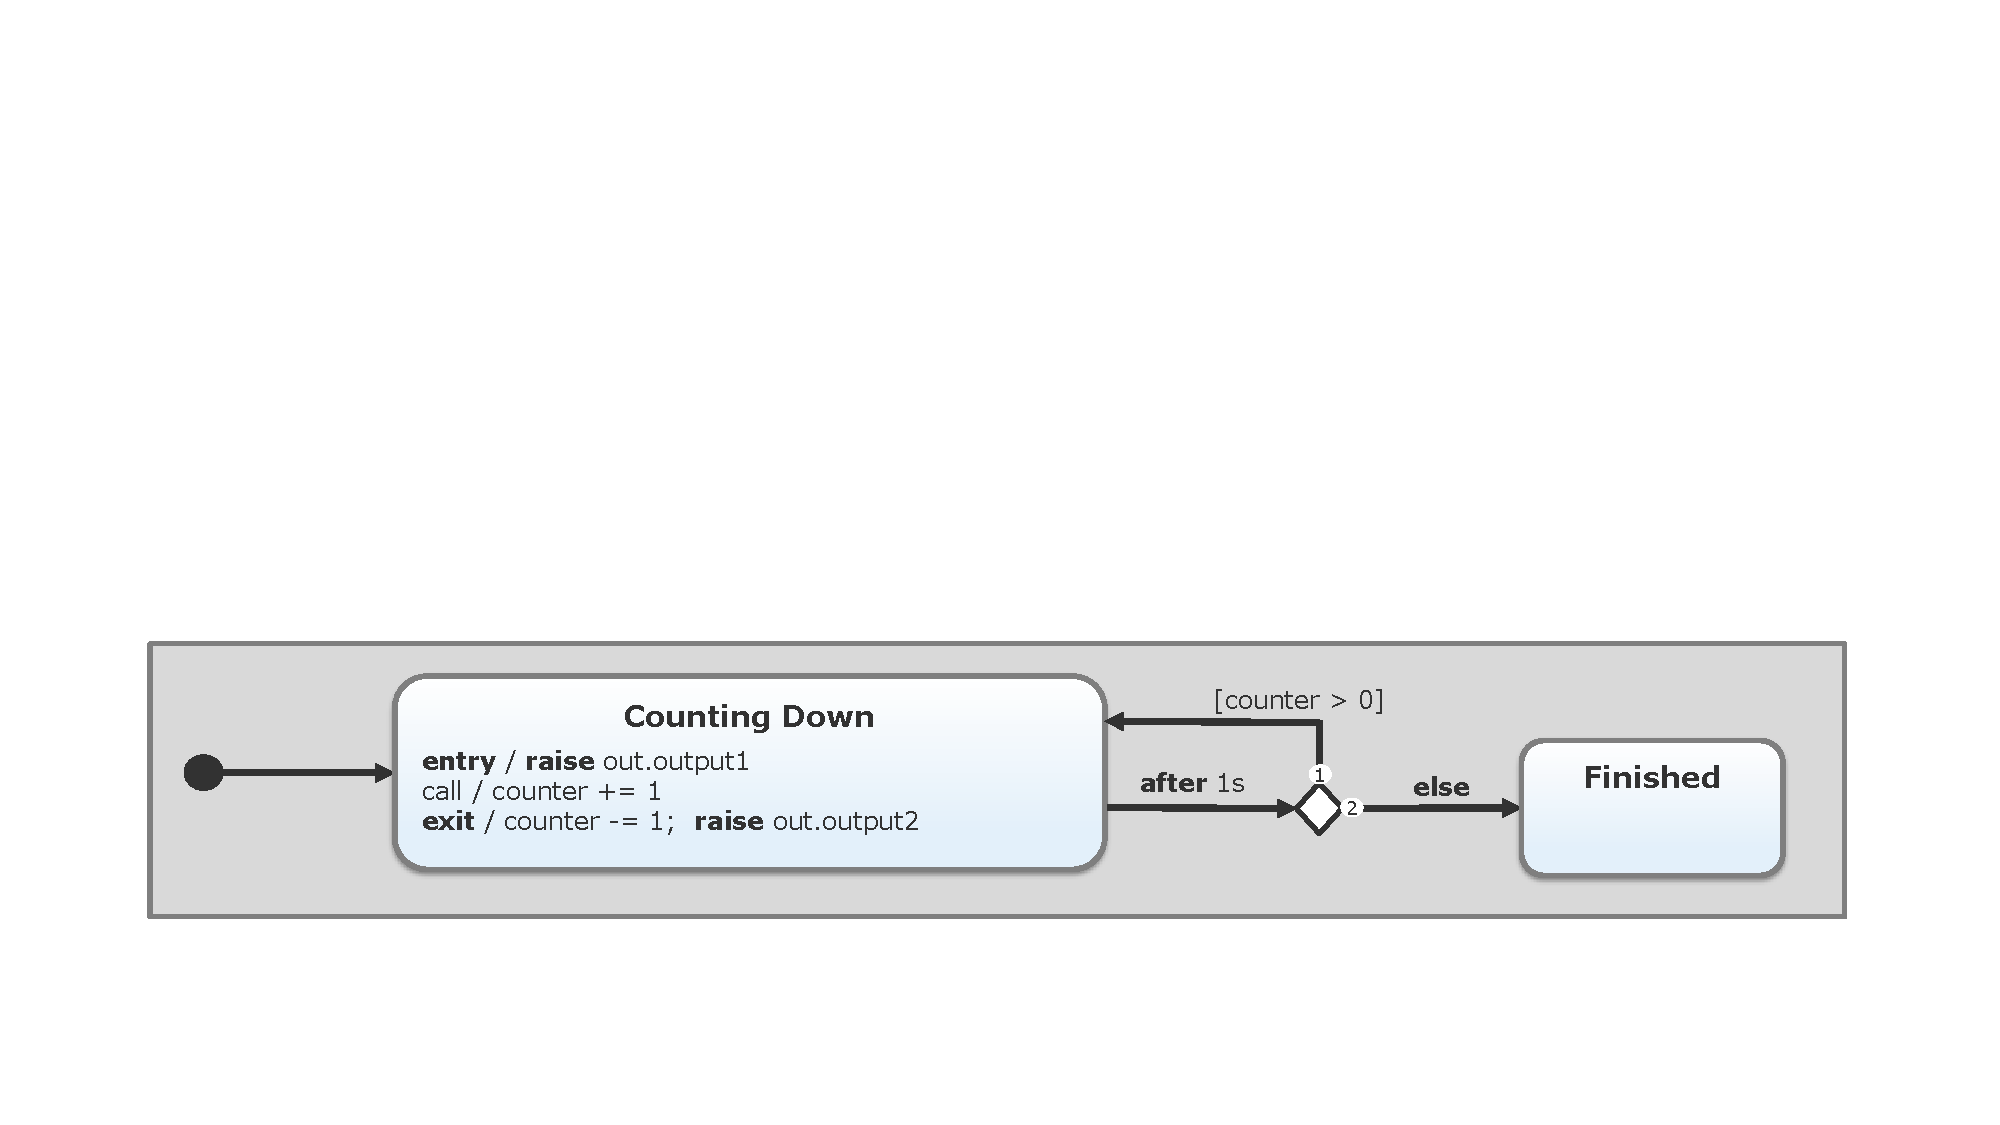
\includegraphics[width=1\textwidth]{syntax_reaktionen}
\end{center}



\subsection{Definitionsbereich}

Ein YAKINDU Statechart hat einen zusätzlichen Definitionsbereich, in dem alle für die Reaktionen benötigten Elemente definiert werden können. Das beinhaltet insbesondere eingehende und ausgehende Ereignisse sowie Operationen, die beispielsweise in Guards aufgerufen werden können. 
Dies entspricht in etwa dem Ein- und Ausgabealphabet eines erweiterten Automaten bzw. dem Klassendiagramm zu einem UML-Zustandsdiagramm. Für diese Aufgabenstellung ist der entsprechende Teil des Definitionsbereiches fest vorgegeben und \textbf{darf nicht verändert werden}.

Außerdem können im Definitionsbereich interne Ereignisse (die per \enquote{raise} aufgerufen und als Trigger empfangen werden können) zur Synchronisation sowie interne Variablen definiert werden.
Dieser mit \enquote{internal} markierte Teil des Definitionsbereiches darf für die Lösung von \docProjectTitle{} um eigene Ereignisse und Variablen ergänzt werden.

Der Definitionsbereich ermöglicht YAKINDU SCT die strikte Syntaxprüfung bei den Reaktionen.
